% !TeX program = xelatex
\documentclass[12pt,letterpaper]{extarticle}
\newcommand{\ReportTitle}{การออกแบบคลังข้อมูลเพื่อวิเคราะห์การลานิสิตตามบทบาทผู้ใช้}
\newcommand{\ReportSubtitle}{Role-Based Data Warehouse Design for Student Leave Analytics}
\newcommand{\ReportAuthors}{%
  \begin{tabular}{@{}ll@{}}
    นายจิรภัทร แซ่ลี้ & 6620501311\\[6pt]
    นายกานตภัท อาจหาญ & 6620503349\\[6pt]
    นายธนวัฒน์ แซ่จึง & 6620503403\\[6pt]
    นายศุภกร ลีลาธนางกุล & 6620503578
\end{tabular}}
\newcommand{\ReportInstitution}{ภาควิชาวิศวกรรมคอมพิวเตอร์\\คณะวิศวกรรมศาสตร์ กำแพงแสน\\มหาวิทยาลัยเกษตรศาสตร์ วิทยาเขตกำแพงแสน}
\newcommand{\ReportDate}{29 ตุลาคม พ.ศ. 2569}
\newif\ifReportMode\ReportModetrue
\newif\ifShowAbstract\ShowAbstractfalse
\newif\ifShowContents\ShowContentstrue
\newif\ifShowTables\ShowTablestrue
\newif\ifShowFigures\ShowFigurestrue

\usepackage{graphicx}
\usepackage{iftex}
\ifXeTeX\else
\PackageError{basic-latex}{This template requires XeLaTeX}{Run scripts/build.ps1 or select XeLaTeX.}
\fi
\usepackage{fontspec}
\usepackage{geometry}
\usepackage{fancyhdr}
\usepackage{float}
\usepackage{hyperref}
\usepackage{enumitem}
\usepackage{datetime2}
\usepackage{indentfirst}
\usepackage[table]{xcolor}
\usepackage{listings}
\usepackage{booktabs}
\usepackage{tabularx}
\usepackage{array}
\usepackage{tikz}
\usepackage{needspace}
\usepackage{titlesec}
\usepackage{setspace}
\usepackage{tocloft}
\usepackage{caption}
\usepackage[most]{tcolorbox}

\usetikzlibrary{arrows.meta,positioning,shapes.geometric}

% ---------------- Page Setup ----------------
\geometry{
  letterpaper,
  margin=2.5cm,
  headheight=20pt,
  headsep=10pt,
  footskip=0.5in
}

% ---------------- Thai Font ----------------
\setmainfont[
  Path=fonts/THSarabun/,
  BoldFont=THSarabun-Bold.ttf,
  ItalicFont=THSarabun-Italic.ttf,
  BoldItalicFont=THSarabun-BoldItalic.ttf
]{THSarabun.ttf}

% ---------------- Code Font ----------------
\setmonofont[
  Path=fonts/JetBrainMono/,
  BoldFont=JetBrainsMono-SemiBold.ttf,
  ItalicFont=JetBrainsMono-Italic.ttf,
  BoldItalicFont=JetBrainsMono-SemiBoldItalic.ttf
]{JetBrainsMono-Regular.ttf}
% Keep each inline identifier intact; use the same mono family as listings.
\RenewDocumentCommand{\texttt}{m}{\mbox{\ttfamily\fontsize{10pt}{14pt}\selectfont #1}}

% ---------------- Thai Date ----------------
\newcommand{\thaimonth}[1]{
  \ifcase#1\or
  มกราคม\or กุมภาพันธ์\or มีนาคม\or เมษายน\or
  พฤษภาคม\or มิถุนายน\or กรกฎาคม\or สิงหาคม\or
  กันยายน\or ตุลาคม\or พฤศจิกายน\or ธันวาคม
  \fi
}

\newcommand{\thaidate}{
  \number\day\space
  \thaimonth{\month}\space
  พ.ศ. \number\numexpr\year+543\relax
}

% รองรับการตัดคำภาษาไทย
\XeTeXlinebreaklocale "th"
\XeTeXlinebreakskip = 0pt plus 0.6pt minus 0.1pt
\XeTeXlinebreakpenalty = 100

% ลดช่องไฟที่กว้างผิดปกติเมื่อจัดข้อความภาษาไทยแบบชิดขอบ
\tolerance=1800
\emergencystretch=1.5em
\hyphenpenalty=10000
\exhyphenpenalty=10000

% ---------------- Paragraph Setup ----------------
\makeatletter
\renewcommand\normalsize{\@setfontsize\normalsize{13pt}{19.5pt}}
\makeatother
\normalsize
\setstretch{1.0}
\leftskip=0pt
\rightskip=0pt
\parfillskip=0pt plus 1fil
% Keep explicit spaces in mixed Thai/English prose from stretching excessively.
\spaceskip=0.25em plus 0.05em minus 0.05em
\raggedbottom
\setlength{\parindent}{0.5in}
\setlength{\parskip}{0pt}
\setlist[itemize]{itemsep=0pt, topsep=3pt, parsep=0pt}
\setlist[enumerate]{itemsep=0pt, topsep=3pt, parsep=0pt}

% ---------------- Heading Setup ----------------
\renewcommand{\contentsname}{สารบัญ}
\renewcommand{\listfigurename}{สารบัญภาพ}
\renewcommand{\listtablename}{สารบัญตาราง}
\renewcommand{\figurename}{ภาพที่}
\renewcommand{\tablename}{ตารางที่}
\DeclareCaptionFont{reportcaption}{\fontsize{12pt}{18pt}\selectfont}
\captionsetup{labelsep=space,font=reportcaption,labelfont=bf,justification=raggedright,singlelinecheck=false}
\captionsetup[table]{position=top,skip=6pt}
\captionsetup[figure]{position=bottom,skip=6pt}
\DeclareCaptionType{codecaption}[โค้ดที่][สารบัญโค้ด]
\captionsetup[codecaption]{position=top,skip=6pt,hypcap=false}
\ifReportMode
\renewcommand{\cftsecpresnum}{บทที่~}
\fi
\setlength{\cftsecnumwidth}{4.2em}
\renewcommand{\cftfigpresnum}{ภาพที่~}
\setlength{\cftfignumwidth}{4.2em}
\renewcommand{\cfttabpresnum}{ตารางที่~}
\setlength{\cfttabnumwidth}{4.6em}
\renewcommand{\cftsecdotsep}{1.5}
\renewcommand{\cftsubsecdotsep}{1.5}
\renewcommand{\cftfigdotsep}{1.5}
\renewcommand{\cfttabdotsep}{1.5}

\renewcommand{\cfttoctitlefont}{\hfill\bfseries\fontsize{20pt}{24pt}\selectfont}
\renewcommand{\cftaftertoctitle}{\hfill}
\renewcommand{\cftloftitlefont}{\hfill\bfseries\fontsize{20pt}{24pt}\selectfont}
\renewcommand{\cftafterloftitle}{\hfill}
\renewcommand{\cftlottitlefont}{\hfill\bfseries\fontsize{20pt}{24pt}\selectfont}
\renewcommand{\cftafterlottitle}{\hfill}

\titleformat{\section}[block]
{\centering\bfseries\fontsize{20pt}{24pt}\selectfont}
{\ifReportMode บทที่ \fi\thesection}
{0.6em}
{}
\titlespacing*{\section}{0pt}{0pt}{0.8\baselineskip}

\titleformat{\subsection}[hang]
{\bfseries\fontsize{16pt}{21pt}\selectfont}
{\thesubsection}
{0.6em}
{}
\titlespacing*{\subsection}{0pt}{0.8\baselineskip}{0.25\baselineskip}

\titleformat{\subsubsection}[hang]
{\bfseries\fontsize{14pt}{19pt}\selectfont}
{\thesubsubsection}
{0.6em}
{}
\titlespacing*{\subsubsection}{0pt}{0.6\baselineskip}{0.2\baselineskip}

% ---------------- Image Path ----------------
\graphicspath{{images/}}

% ---------------- Header and Footer ----------------
\pagestyle{fancy}
\fancyhf{}
\renewcommand{\headrulewidth}{0pt}
\fancyhead[L]{}
\fancyfoot[C]{\thepage}
\fancypagestyle{plain}{%
  \fancyhf{}
  \renewcommand{\headrulewidth}{0pt}
  \fancyhead[L]{}
  \fancyfoot[C]{\thepage}
}

\renewcommand{\sectionmark}[1]{\markboth{บทที่ \thesection\quad #1}{}}

% ---------------- Hyperlink Setup ----------------
\hypersetup{
  colorlinks=true,
  linkcolor=black,
  urlcolor=blue
}

% ---------------- Color Setup ----------------
\definecolor{primaryblue}{HTML}{2196F3}
\definecolor{lightblue}{HTML}{E3F2FD}
\definecolor{codebackground}{HTML}{F6F8FA}
\definecolor{codeborder}{HTML}{D0D7DE}
\definecolor{codetext}{HTML}{111827}
\definecolor{codemuted}{HTML}{64748B}
\definecolor{codegreen}{HTML}{52525B}

\definecolor{codekeyword}{HTML}{8B46FF}
\definecolor{codestring}{HTML}{008577}
\definecolor{codefunction}{HTML}{005CC5}

% ---------------- Code Listing Setup ----------------
\lstset{
  basicstyle=\color{codetext}\ttfamily\fontsize{10pt}{14pt}\selectfont,
  backgroundcolor=\color{codebackground},
  frame=single,
  rulecolor=\color{codeborder},
  frameround=tttt,
  framesep=0.45cm,
  keywordstyle=\color{codetext}\bfseries,
  commentstyle=\color{codegreen},
  stringstyle=\color{codemuted},
  showstringspaces=false,
  breaklines=false,
  breakatwhitespace=true,
  columns=fullflexible,
  keepspaces=true,
  tabsize=2,
  xleftmargin=0cm,
  xrightmargin=0cm,
  framexleftmargin=0.15cm,
  framexrightmargin=0.15cm,
  framextopmargin=0.35cm,
  framexbottommargin=0.35cm,
  aboveskip=0.8em,
  belowskip=0.8em
}

% ---------------- TikZ Setup ----------------
\tikzset{
  flow/.style={
    rectangle,
    rounded corners=3pt,
    draw=primaryblue,
    fill=lightblue,
    minimum width=3.2cm,
    minimum height=1cm,
    align=center
  },
  decision/.style={
    diamond,
    aspect=2.2,
    draw=primaryblue,
    fill=lightblue,
    minimum width=3cm,
    minimum height=1.1cm,
    align=center
  },
  line/.style={
    -{Latex[length=3mm]},
    thick,
    draw=gray!70
  }
}

\lstdefinelanguage{JavaScript}{
  keywords={
    const, let, var, function, return, if, else,
    for, while, do, switch, case, break, continue,
    true, false, null, undefined, new, class,
    import, export, from, async, await, try, catch,
    finally, throw, typeof, instanceof
  },
  morekeywords=[2]{prepare,run,get,all,exec,Number,Set},
  keywordstyle=\color{codetext}\bfseries,
  sensitive=true,
  comment=[l]{//},
  morecomment=[s]{/*}{*/},
  commentstyle=\color{codegreen},
  morestring=[b]',
  morestring=[b]",
  morestring=[b]`,
  stringstyle=\color{codemuted}
}

\lstdefinelanguage{JSON}{
  keywords={true,false,null},
  keywordstyle=\color{primaryblue}\bfseries,
  sensitive=true,
  morestring=[b]",
  stringstyle=\color{orange!80!black}
}

% ---------------- Code Block: light rounded panel ----------------
\newtcblisting{codeblock}[1]{
  enhanced,
  unbreakable,
  listing only,
  colback=codebackground,
  colframe=codeborder,
  boxrule=0.75pt,
  arc=4.5pt,
  outer arc=4.5pt,
  boxsep=0pt,
  left=4mm,
  right=4mm,
  top=3mm,
  bottom=3mm,
  before skip=0pt,
  after skip=3pt,
  listing options={
    language=#1,
    basicstyle=\ttfamily\fontsize{10pt}{14pt}\selectfont\color{codetext},
    keywordstyle=\color{codekeyword},
    keywordstyle={[2]\color{codefunction}},
    commentstyle=\color{codemuted},
    stringstyle=\color{codestring},
    backgroundcolor=\color{codebackground},
    frame=none,
    framesep=0pt,
    xleftmargin=0pt,
    xrightmargin=0pt,
    framexleftmargin=0pt,
    framexrightmargin=0pt,
    aboveskip=0pt,
    belowskip=0pt,
    numbers=none,
    showstringspaces=false,
    breaklines=false,
    breakatwhitespace=true,
    columns=fullflexible,
    keepspaces=true,
    tabsize=2
  }
}

% ---------------- Shared document helpers ----------------
\setsansfont[
  Path=fonts/THSarabun/,
  BoldFont=THSarabun-Bold.ttf,
  ItalicFont=THSarabun-Italic.ttf,
  BoldItalicFont=THSarabun-BoldItalic.ttf
]{THSarabun.ttf}
\usepackage{longtable}
% URLs remain whole and start on a separate line in references.
\usepackage{etoolbox}
\AtBeginEnvironment{longtable}{\small\setlength{\tabcolsep}{4pt}}
\renewcommand{\refname}{เอกสารอ้างอิง}
\newcommand{\code}[1]{\texttt{\detokenize{#1}}}
\newcommand{\tablecode}[1]{\mbox{\ttfamily\fontsize{10pt}{14pt}\selectfont\detokenize{#1}}}
\lstdefinelanguage{PlainText}{}
\hypersetup{pdftitle={\ReportTitle},citecolor=black}
\newcommand{\reporturl}[1]{\par\nobreak\noindent\mbox{\href{#1}{\ttfamily\fontsize{10pt}{14pt}\selectfont\detokenize{#1}}}\par}
\setlength{\heavyrulewidth}{0.5pt}
\setlength{\lightrulewidth}{0.35pt}
\definecolor{tableheader}{HTML}{E9EDF2}

% Use a local left-aligned paragraph when long identifiers make justification ugly.
\newenvironment{mixedprose}{\par\begingroup\rightskip=0pt plus 1fil}{\par\endgroup}
% A code panel and its caption remain together; do not nest this inside a float.
\newenvironment{codepanel}[1]{%
  \par\addvspace{8pt}\noindent
  \begin{minipage}{\linewidth}%
    \captionof{codecaption}{#1}\nopagebreak
  }{%
  \end{minipage}\par\addvspace{6pt}%
}
\newcommand{\frontmatterpages}{%
  \pagenumbering{roman}%
  \renewcommand{\thepage}{\ifcase\value{page}\or ก\or ข\or ค\or ง\or จ\or ฉ\or ช\or ซ\or ฌ\or ญ\or ฎ\or ฏ\or ฐ\or ฑ\or ฒ\or ณ\else\arabic{page}\fi}%
}
\newcommand{\nextchapter}{\ifReportMode\clearpage\fi}

\usepackage{cite}
\usepackage{pdflscape}
\XeTeXgenerateactualtext=1
\captionsetup[figure]{justification=centering}
\setlength{\cftbeforesecskip}{4pt}
\begin{document}
\begin{titlepage}
  \thispagestyle{empty}
  \centering
  \vspace*{1cm}
  {\fontsize{20pt}{26pt}\selectfont รายงาน\par}
  \vspace{0.6cm}
  {\bfseries\fontsize{20pt}{26pt}\selectfont\ReportTitle\par}
  \vspace{0.8cm}
  {\fontsize{16pt}{22pt}\selectfont\ReportSubtitle\par}
  \vspace{1.5cm}
  {\fontsize{16pt}{22pt}\selectfont ผู้จัดทำ\par}
  \vspace{0.5cm}
  {\fontsize{14pt}{21pt}\selectfont\ReportAuthors\par}
  \vspace{1.5cm}
  {\fontsize{14pt}{21pt}\selectfont\ReportInstitution\par}
  \vfill
  {\fontsize{14pt}{21pt}\selectfont\ReportDate\par}
  \vspace{1cm}
\end{titlepage}

\frontmatterpages
\tableofcontents
\clearpage
\listoftables
\clearpage
\listoffigures
\clearpage
\pagenumbering{arabic}
\section{บทนำ}
ข้อมูลการลานิสิตสามารถสะท้อนรูปแบบการขาดเรียนในแต่ละช่วงเวลา รายวิชา และกลุ่มนิสิต แต่ฐานข้อมูลที่รองรับงานประจำวันไม่ได้จัดรูปแบบมาเพื่อเปรียบเทียบหลายภาคการศึกษาโดยตรง คลังข้อมูลจึงทำหน้าที่รวบรวมบริบทที่จำเป็นและกำหนดหน่วยการวัดให้สอดคล้องกัน เพื่อให้ผู้ใช้แต่ละบทบาทมองข้อมูลจากรายละเอียดของตนไปถึงภาพรวมระดับคณะได้\cite{repo,warehouse}

วัตถุประสงค์ของบทความประกอบด้วยการอธิบายสถาปัตยกรรมคลังข้อมูล การกำหนดระดับรายละเอียดของข้อเท็จจริงและมิติ การเชื่อมข้อมูลเพื่อวิเคราะห์ และคำถามที่มุมมองแต่ละบทบาทตอบได้ ขอบเขตจำกัดอยู่ที่สถิติการลาและผลกระทบต่อการเรียน โดยไม่มีการนำภาพหน้าจอมาใช้ประกอบ

หลักฐานหลักคือโค้ดใน \nolinkurl{apps/api} และ \nolinkurl{apps/web} ของโครงการ ส่วนเอกสารสคีมาใช้ประกอบการอธิบายความสัมพันธ์ ไม่ถือว่าสคีมาที่ออกแบบหรือหน้ารายงานที่มีอยู่เป็นหลักฐานว่าข้อมูลจริงครบถ้วนหรือผ่านการประเมินประสิทธิภาพแล้ว

\nextchapter
\section{แนวคิดการออกแบบคลังข้อมูล}
\subsection{การแยกงานวิเคราะห์จากงานประจำวัน}
ฐานข้อมูลต้นทางเก็บรายการและข้อมูลประกอบตามเหตุการณ์ ส่วนคลังข้อมูลจัดเก็บข้อมูลที่ผ่านการแปลงและเชื่อมรหัสอ้างอิงเพื่ออ่านซ้ำในหลายรายงาน เส้นทางข้อมูลประกอบด้วยการสกัด การแปลง และการโหลด หรือ ETL จากนั้นบริการรายงานจำกัดขอบเขตข้อมูลก่อนจัดรูปแบบสำหรับหน้าเว็บ

\subsection{ข้อเท็จจริง มิติ และระดับรายละเอียด}
ข้อเท็จจริงเก็บเหตุการณ์และค่าที่วัดได้ ส่วนมิติเก็บคุณลักษณะสำหรับจัดกลุ่มและกรองข้อมูล การกำหนดระดับรายละเอียดหรือ grain ต้องมาก่อนการเลือกกราฟ เพราะใบลาเดียวอาจสัมพันธ์กับหลายรายวิชา หลายกลุ่มเรียน และหลายผู้สอน การเชื่อมทุกความสัมพันธ์แล้วรวมวันลาทันทีทำให้ยอดภาพรวมสูงเกินจริง

แบบจำลองรุ่นใหม่จึงมีลักษณะกลุ่มดาวข้อเท็จจริง โดยใช้หลายตารางข้อเท็จจริงร่วมมิติเดียวกัน แยกตารางเชื่อมสำหรับความสัมพันธ์หลายต่อหลาย และแยกความเป็นเจ้าของรายวิชาออกจากสังกัดนิสิตและบุคลากร เพื่อไม่ให้รายงานต่างระดับใช้คำว่า ``ภาควิชา'' แทนข้อมูลคนละความหมาย

\subsection{บริบทในอดีตและสิทธิ์ปัจจุบัน}
สังกัด หลักสูตร และที่ปรึกษา ณ เวลายื่นเป็นบริบทเชิงวิเคราะห์ ขณะที่รายชื่อผู้ที่ผู้ใช้เข้าถึงได้ต้องตรวจจากสิทธิ์และความสัมพันธ์ปัจจุบัน การมีรหัสบุคคลอยู่ในคลังข้อมูลไม่ได้ให้สิทธิ์เปิดดูข้อมูลของบุคคลนั้นโดยอัตโนมัติ

\nextchapter
\section{โครงสร้างและวิธีออกแบบ}
\subsection{สถาปัตยกรรมข้อมูล}
โค้ดมีโครงสร้าง \nolinkurl{wh_*} เดิมใน Prisma และโครงสร้าง \nolinkurl{dw_*} รุ่นใหม่ในชุด ETL อยู่ร่วมกัน บทความนี้ใช้รุ่นใหม่เป็นแกน เพราะแยกใบลาออกจากรายวิชาและรองรับบริบทหน่วยงานชัดเจน การนับแถวในตารางเดิมจึงไม่ควรนำมาเทียบกับจำนวนใบลาในรุ่นใหม่โดยไม่ตรวจ grain\cite{model,etl}

ชุด ETL อยู่ใน \nolinkurl{apps/api/scripts/warehouse-etl} โดยแยกโมดูลสกัด แปลง ตรวจสอบ และโหลดข้อมูล บริการ \nolinkurl{WarehouseLiveService} อ่านตารางรุ่นใหม่และจัดขอบเขตตามผู้ใช้ ส่วน \nolinkurl{live-report-data.ts} แปลงชุดข้อมูลเป็นโครงสร้างที่หน้ารายงานใช้งานได้

\subsection{ตารางข้อเท็จจริง}
\textbf{ระดับใบลา:} \nolinkurl{dw_fact_leave_request} กำหนดหนึ่งแถวต่อหนึ่งใบลาจากระบบต้นทาง มีรหัสต้นทางเพื่อป้องกันรายการซ้ำ เชื่อมนิสิต ภาคการศึกษา ประเภทลา หน่วยงาน หลักสูตร และที่ปรึกษา เก็บวันเริ่ม วันสิ้นสุด จำนวนวันลา ชั้นปี และข้อมูลกำกับรอบนำเข้า ยอดรวมระดับนิสิต ภาควิชา หรือคณะควรเริ่มจากตารางนี้

\textbf{ระดับใบลากับกลุ่มเรียน:} \nolinkurl{dw_fact_leave_subject} มีคีย์ร่วมระหว่างใบลากับ offering หนึ่งใบลาจึงมีได้หลายแถว เก็บจำนวนวันเรียน ครั้งเรียน และชั่วโมงเรียนที่ได้รับผลกระทบเมื่อมีข้อมูลเพียงพอ ใช้วิเคราะห์รายวิชาและกลุ่มเรียน ไม่ใช้จำนวนแถวแทนจำนวนใบลาของทั้งคณะ

ตัวอย่างเชิงอธิบาย: ใบลา A มี 2 วันและเกี่ยวข้องกับ 3 รายวิชา ยอดภาพรวมเท่ากับ 1 ใบและ 2 วัน ส่วนความสัมพันธ์รายวิชาเท่ากับ 3 รายการ หากผู้สอนร่วมมี 2 คน จำนวนแถวหลังเชื่อมอาจเพิ่มอีก การรวมต้องกลับไปที่คีย์ใบลาหรือคีย์ใบลา--offering ตามคำถาม ตัวอย่างนี้มิใช่สถิติจากฐานข้อมูลจริง

\subsection{มิติและตารางเชื่อม}
มิตินิสิตและบุคลากรระบุตัวตน มิติประเภทลาจัดกลุ่มเหตุการณ์ มิติภาคการศึกษากำหนดลำดับเทอมและปีสำหรับเปรียบเทียบ แม้เทอมนั้นไม่มีใบลา มิติรายวิชาแยกรหัสและรุ่นข้อมูลวิชา ส่วนมิติ offering ระบุรายวิชา เทอม กลุ่มเรียน และชนิดกลุ่มเรียน

มิติคณะ ภาควิชา และหลักสูตรอธิบายโครงสร้างองค์กร โดยสังกัดนิสิตใน fact แยกจากเจ้าของรายวิชาในมิติ subject/offering และสังกัดอาจารย์ ตาราง \nolinkurl{dw_snapshot_student_term} รองรับบริบทนิสิตรายเทอม ส่วนตารางเชื่อมบุคลากรกับหน่วยงานรายเทอมรองรับการจัดกลุ่มบุคลากร

ตาราง \nolinkurl{dw_bridge_offering_lecturer} รองรับผู้สอนร่วมของกลุ่มเรียน และ \nolinkurl{dw_bridge_leave_subject_lecturer} เก็บความสัมพันธ์ผู้สอนกับรายวิชาในใบลา การกรองรายงานของผู้สอนจึงต้องระวังไม่ทำให้ใบลาเดียวถูกนับซ้ำตามจำนวนผู้สอน

\subsection{กระบวนการ ETL และคุณภาพข้อมูล}
การสกัดรวบรวมรายการต้นทางและข้อมูลอ้างอิง การแปลงจัดรูปแบบรหัส วันที่ ประเภทลา และความสัมพันธ์ให้เป็นแบบเดียวกัน การโหลดแก้ไขหรือเพิ่มข้อมูลด้วยคีย์ต้นทาง และบันทึกรอบนำเข้าไว้ใน \nolinkurl{dw_load_batch} ส่วน \nolinkurl{dw_data_issue} รองรับการติดตามปัญหาคุณภาพข้อมูล

กระบวนการปัจจุบันเป็นการประมวลผล snapshot ทั้งชุดในหน่วยความจำ แล้วเขียนเป้าหมายใน transaction เดียว การประกาศรอบสำเร็จจึงผูกกับข้อมูลที่เขียนครบ ไม่ใช่กระบวนการ CDC หรือการส่งข้อมูลทันทีทุกเหตุการณ์ การจัดการรายการที่หายจากต้นทางต้องใช้ reconciliation ตามเงื่อนไขที่กำหนด

รหัสนิสิต รายวิชา และรหัสต้นทางต้องคงรูปสตริงเพื่อรักษาเลขศูนย์นำหน้าและหลีกเลี่ยงเลขขนาดใหญ่สูญเสียความแม่นยำ การจับคู่สังกัด หลักสูตร และบุคลากรต้องมีข้อมูลอ้างอิงที่ตรวจสอบได้ ค่าที่ไม่ทราบต้องแยกจากศูนย์ โดยเฉพาะผลกระทบต่อการเรียนที่ยังไม่มีตารางเรียนครบถ้วน

\subsection{นิยามตัวชี้วัด}
จำนวนใบลาคือจำนวนคีย์ใบลาที่ไม่ซ้ำในขอบเขตที่เลือก จำนวนผู้ลาคือจำนวนนิสิตไม่ซ้ำ ส่วนวันลารวมเป็นผลรวม \nolinkurl{request_days} จาก fact ระดับใบลา การใช้ผลรวมค่าที่ไม่ซ้ำตามตัวเลขวันลาไม่ถูกต้อง เพราะหลายใบอาจมีจำนวนวันเท่ากัน

วันลาตามปฏิทินไม่เท่ากับวันเรียนหรือชั่วโมงเรียนที่ขาด การวัดผลกระทบรายวิชาต้องอาศัยวันที่เรียนจริง ระยะเวลาคาบ และความสัมพันธ์กับใบลา การรวมชั่วโมงหลายวิชามีหน่วยเป็นชั่วโมงเรียนที่ได้รับผลกระทบ ไม่ใช่เวลาตามปฏิทินของนิสิต

ค่าเฉลี่ยต่อเทอมต้องใช้จำนวนเทอมที่เลือกเป็นตัวหาร รวมเทอมยอดศูนย์ สำหรับ box plot ของรายวิชา หน่วยตัวอย่างเป็นยอดรวมของรายวิชาต่อเทอมในช่วงที่เลือก มิใช่ความยาวของใบลาแต่ละใบ และต้องแสดงกรณีไม่มีตัวอย่างอย่างชัดเจน

\subsection{ขอบเขตการเข้าถึง}
บริการรายงานตรวจตัวตนและบทบาทจากฝั่งเซิร์ฟเวอร์ แล้วใช้รายชื่อนิสิตในที่ปรึกษา รายวิชาและกลุ่มเรียนที่สอน หรือหน่วยงานปัจจุบันเป็นขอบเขต ผู้บริหารเข้าถึงหน่วยงานภายในคณะที่ได้รับสิทธิ์ ส่วนเจ้าหน้าที่ใช้ขอบเขตภาควิชาจากบัญชีในโค้ดที่ตรวจ ไม่อนุมานว่ามีสิทธิ์ทุกคณะ การเปิดรายละเอียดต้องรักษาขอบเขตเดียวกับหน้าสรุป\cite{service}

ภาพสคีมาจากบทความต้นฉบับแสดงในภาคผนวก ข โดยภาพที่~\ref{fig:warehouse-schema-overview} แสดงการจัดกลุ่มตาราง และภาพรายละเอียดแสดงคีย์กับคอลัมน์สำหรับอ่านประกอบแบบจำลอง

\nextchapter
\section{มุมมองรายงานตามบทบาท}
เนื้อหาส่วนนี้อธิบายคำถามที่โครงสร้างข้อมูลและหน้ารายงานรองรับจากการตรวจโค้ด มิใช่ผลทดลองกับผู้ใช้จริง ตัวกรองร่วมประกอบด้วยภาคการศึกษาหรือช่วงเทอม ประเภทลา และช่วงจำนวนวันลา โดยแต่ละหน้ามีตัวกรองรายละเอียดเพิ่มเติม\cite{pages}

\subsection{นิสิต: รูปแบบการลาของตนเอง}
มุมมองนิสิตจำกัดข้อมูลของตนเอง ตอบได้ว่าแต่ละเทอมมีใบลาและวันลากี่รายการ ประเภทใดมีสัดส่วนมาก และรายวิชาใดเกี่ยวข้องกับการลามากที่สุด หน้าเว็บมีภาพรวมและตารางรายเทอม รวมทั้งรายละเอียดรายวิชา การเปรียบเทียบใช้มิติเทอม ประเภทลา และ subject/offering ร่วมกับ fact ทั้งสองระดับ

ข้อมูลนี้ช่วยให้นิสิตทบทวนรูปแบบการเข้าเรียนของตน แต่ไม่เพียงพอสำหรับสรุปอัตราขาดเรียนหรือสิทธิ์เข้าสอบ หากยังไม่มีจำนวนครั้งเรียนทั้งหมดและเกณฑ์ของแต่ละวิชา

\subsection{อาจารย์ที่ปรึกษา: กลุ่มนิสิตในความดูแล}
มุมมองที่ปรึกษาตอบว่าในนิสิตที่ดูแล ชั้นปีใดมีการลาสูง ใครบ้างมีจำนวนใบลาหรือวันลาสูง และรูปแบบเปลี่ยนไปอย่างไรระหว่างเทอม หน้าเว็บมีกราฟเปรียบเทียบชั้นปี สัดส่วน ตารางสรุป Top 10 และการค้นหารหัสนิสิต พร้อมเปิดรายละเอียดรายบุคคล

ขอบเขตกลุ่มนิสิตอ้างอิงความสัมพันธ์ปัจจุบันของที่ปรึกษา ขณะที่มิติที่ปรึกษาใน fact ใช้บริบท ณ เวลายื่น การจัดอันดับที่ปรึกษาในภาพรวมจึงต้องระบุนิยามให้ต่างจากการติดตามรายชื่อนิสิตที่ตนดูแลอยู่ในปัจจุบัน

\subsection{อาจารย์ผู้สอน: ผลกระทบต่อรายวิชา}
มุมมองผู้สอนตอบว่ารายวิชาหรือกลุ่มเรียนที่สอนมีการลาเท่าใด เทอมใดสูงกว่าช่วงอื่น และนิสิตคนใดมีการลาในรายวิชานั้น หน้าเว็บมีกราฟเปรียบเทียบ สัดส่วน ตารางรายวิชา แนวโน้มรายเทอม การกระจายของยอดรายวิชา และรายละเอียดรายวิชากับวันเรียน

หน่วยการวิเคราะห์หลักคือ offering และความสัมพันธ์ใบลากับ offering โดยกรองตามสิทธิ์ผู้สอนปัจจุบัน การมีผู้สอนร่วมต้องไม่เพิ่มยอดรวมรายวิชา และยอดจากหลายวิชาไม่ควรรวมแล้วเรียกว่าใบลารวมของนิสิตโดยไม่ตัดคีย์ซ้ำ

\subsection{หัวหน้าภาควิชา: นิสิตและรายวิชาในภาค}
มุมมองนี้ตอบได้สองแกน ได้แก่ภาพรวมการลาของนิสิตในภาค และผลกระทบต่อรายวิชาที่ภาคเป็นเจ้าของ หน้าเว็บรองรับการเปรียบเทียบตามที่ปรึกษา ชั้นปี ผู้สอน และรายวิชา มีตารางนิสิต การค้นหา และรายละเอียดผลกระทบตามวิชา

แกนนิสิตใช้สังกัดนิสิต ส่วนแกนรายวิชาใช้เจ้าของวิชา นิสิตต่างภาคที่เรียนวิชาของภาคจึงอาจอยู่ในรายงานรายวิชาโดยไม่อยู่ในภาพรวมนิสิตของภาค รายการวิชาในภาคควรรวมวิชายอดศูนย์เมื่อมีบัญชีรายวิชาครบ ไม่เริ่มรายงานจากใบลาที่มีอยู่เพียงอย่างเดียว

\subsection{ผู้บริหาร: ภาพรวมระดับคณะ}
มุมมองผู้บริหารตอบว่าการลากระจายระหว่างภาควิชาอย่างไร หลักสูตรใดมีจำนวนสูง และกลุ่มนิสิตตามที่ปรึกษาใดควรติดตาม หน้าเว็บจัดลำดับภาพรวมตามภาควิชา ต่อด้วยหลักสูตร และที่ปรึกษา พร้อม Top 10 และรายละเอียดภาคภายในคณะที่ได้รับสิทธิ์

จำนวนใบลาเป็นตัวชี้วัดขนาดเหตุการณ์ ยังใช้เปรียบเทียบความเสี่ยงระหว่างภาคโดยตรงไม่ได้ เพราะแต่ละภาคมีจำนวนนิสิตต่างกัน หากต้องการอัตราการลา ต้องเพิ่มตัวหารจากทะเบียนนิสิตที่มีขอบเขตและเทอมตรงกัน การจัดอันดับจึงเป็นจุดเริ่มต้นการตรวจข้อมูล ไม่ใช่ข้อสรุปเชิงสาเหตุ

\subsection{เจ้าหน้าที่: ติดตามภาพรวมภายในภาค}
มุมมองเจ้าหน้าที่มีกราฟเปรียบเทียบตามอาจารย์ สัดส่วน ตารางสรุป และจำนวนการลาแยกชั้นปี ใช้ตอบว่ากลุ่มนิสิตภายใต้ที่ปรึกษาคนใดมีการลามากในช่วงที่เลือก และควรตรวจรายละเอียดกลุ่มใดเพิ่มเติม โดยใช้ขอบเขตภาควิชาของบัญชีตามบริการปัจจุบัน

\subsection{สถานะการเชื่อมข้อมูลที่ตรวจพบ}
บริการฝั่ง API มีโค้ดอ่าน \nolinkurl{dw_*} และตรวจบทบาท แต่ \nolinkurl{LiveReportProvider} ในเว็บเรียก \nolinkurl{createMockLiveReportData()} จึงยังไม่ยืนยันว่าหน้ารายงานเหล่านี้แสดงคลังข้อมูลจริง การมี service และตัวแปลงข้อมูลอยู่แล้วไม่เท่ากับการต่อข้อมูลครบเส้นทาง

นอกจากนี้ ตัวแปลงบางส่วนแปลงค่าชั่วโมงที่ไม่มีข้อมูลเป็นศูนย์ จึงต้องแยกสถานะความครบถ้วนก่อนใช้สรุปว่าไม่มีผลกระทบ บริการอ่านหลายตารางแบบขนานและมีแคชชุดข้อมูล ขณะที่เวลารอบสำเร็จเป็นข้อมูลกำกับ ความสอดคล้องของทุก query ใน snapshot เดียวกันยังต้องตรวจเพิ่มก่อนอ้างว่ารายงานมีความคงที่ระดับรอบนำเข้า

\nextchapter
\section{สรุปและอภิปราย}
คลังข้อมูลการลานิสิตใช้ข้อเท็จจริงระดับใบลาและระดับใบลากับกลุ่มเรียนร่วมกับมิติกลาง เพื่อรองรับคำถามตั้งแต่พฤติกรรมรายบุคคลถึงภาพรวมระดับคณะ จุดสำคัญของการออกแบบคือการกำหนด grain ให้ชัด แยกบริบทองค์กร และควบคุมการนับซ้ำจากรายวิชาหรือผู้สอนร่วม

มุมมองทั้งหกบทบาทใช้ข้อมูลพื้นฐานร่วมกัน แต่ต่างกันที่ขอบเขตประชากร รายละเอียดที่เปิดดูได้ และวัตถุประสงค์ การใช้ข้อมูลเพื่อการตัดสินใจจึงต้องระบุหน่วยนับ ช่วงเวลา ตัวกรอง และแหล่งข้อมูลกำกับทุกครั้ง

งานที่ควรดำเนินการต่อคือเชื่อมหน้าเว็บกับบริการจริง ตรวจยอดระดับใบลาและรายวิชาเทียบต้นทาง รักษาค่าไม่ทราบให้ต่างจากศูนย์ ตรวจสิทธิ์การเปิดรายละเอียดข้ามบุคคลและข้ามหน่วยงาน รวมถึงทดสอบการอ่านข้อมูลระหว่างเปลี่ยนรอบ ETL ทั้งนี้การจัดทำบทความครั้งนี้ไม่ได้รัน ETL โหลดฐานข้อมูล หรือวัดประสิทธิภาพระบบ จึงไม่มีตัวเลขผลทดลองหรือผลประเมินความพึงพอใจที่ยืนยันได้

\nextchapter
\phantomsection
\addcontentsline{toc}{section}{เอกสารอ้างอิง}
\begin{thebibliography}{9}
\bibitem{repo} ผู้พัฒนาโครงการ, ``KUKPS Engineering Leave Request,'' ซอร์สโค้ดภายในส่วน apps/api และ apps/web, ตรวจเมื่อ 29 ตุลาคม 2569.
\bibitem{warehouse} ผู้พัฒนาโครงการ, ``Report Warehouse v2,'' docs/report-warehouse/README.md และ 01-schema.sql, เอกสารออกแบบภายในโครงการ.
\bibitem{model} ผู้พัฒนาโครงการ, ``Warehouse model,'' apps/api/scripts/warehouse-etl/model.mjs และ apps/api/prisma/warehouse.prisma.
\bibitem{etl} ผู้พัฒนาโครงการ, ``Warehouse ETL,'' apps/api/scripts/warehouse-etl/extract.mjs, transform.mjs และ load.mjs.
\bibitem{service} ผู้พัฒนาโครงการ, ``WarehouseLiveService,'' apps/api/src/warehouse-dashboard/warehouse-live.service.ts.
\bibitem{pages} ผู้พัฒนาโครงการ, ``Role report pages and data adapters,'' apps/web/app/student/report, apps/web/app/user/report, apps/web/lib/live-report-data.ts และ apps/web/components/report/live-report-provider.tsx.
\end{thebibliography}

\clearpage
\appendix
\titleformat{\section}[block]{\centering\bfseries\fontsize{20pt}{24pt}\selectfont}{ภาคผนวก \thesection}{0.6em}{}
\section{สรุปแบบจำลองและหลักฐานจากโค้ด}
\begin{figure}[H]
\centering
\begin{tikzpicture}[node distance=9mm, every node/.style={draw,rounded corners,align=center,font=\normalsize,text width=38mm,minimum height=12mm},>=Stealth]
\node (source) at (0,0) {ข้อมูลต้นทาง\\รายการและข้อมูลอ้างอิง};
\node (etl) at (5.2,0) {ETL\\สกัด แปลง ตรวจ และโหลด};
\node (dw) at (10.4,0) {คลังข้อมูลรุ่นใหม่\\มิติ Fact และ Bridge};
\node (api) at (10.4,-2.2) {บริการรายงาน\\ตรวจตัวตนและขอบเขต};
\node (adapter) at (5.2,-2.2) {ตัวแปลงข้อมูลรายงาน\\สรุปและจัดกลุ่ม};
\node (web) at (0,-2.2) {มุมมอง 6 บทบาท\\กราฟ ตาราง รายละเอียด};
\draw[->] (source)--(etl); \draw[->] (etl)--(dw); \draw[->] (dw)--(api);
\draw[->,dashed] (api)--(adapter); \draw[->] (adapter)--(web);
\end{tikzpicture}
\caption{สถาปัตยกรรมเป้าหมายของรายงาน เส้นประคือการเชื่อมที่ต้องยืนยันเพิ่มเติม เนื่องจาก provider ปัจจุบันใช้ข้อมูลจำลอง ภาพนี้วาดด้วยเวกเตอร์ในเอกสาร}
\end{figure}

\begin{figure}[H]
\centering
\begin{tikzpicture}[every node/.style={draw,rounded corners,align=center,font=\normalsize,text width=39mm,minimum height=13mm},>=Stealth]
\node (request) at (0,0) {Fact: ใบลา\\1 แถวต่อใบลา};
\node (student) at (-5,0) {มิตินิสิตและบุคลากร\\ผู้ลาและที่ปรึกษา};
\node (org) at (5,0) {มิติองค์กรและประเภทลา\\คณะ ภาค หลักสูตร};
\node (term) at (0,2.2) {มิติภาคการศึกษา\\ปี เทอม และลำดับ};
\node (rs) at (0,-2.2) {Fact: ใบลา--กลุ่มเรียน\\1 แถวต่อคู่คีย์};
\node (offering) at (-5,-2.2) {มิติรายวิชาและ Offering\\วิชา เทอม กลุ่มเรียน};
\node (bridge) at (5,-2.2) {ตารางเชื่อมผู้สอน\\รองรับหลายผู้สอน};
\draw[->] (student)--(request); \draw[->] (org)--(request); \draw[->] (term)--(request);
\draw[->] (request)--node[right,draw=none,text width=12mm,minimum height=0mm]{1:N}(rs);
\draw[->] (offering)--(rs); \draw[->] (rs)--(bridge);
\end{tikzpicture}
\caption{แบบจำลองเชิงแนวคิดเฉพาะการวิเคราะห์การลา ลูกศรแสดงการเชื่อมข้อมูล ไม่ใช่ ERD ครบทุกคีย์}
\end{figure}


\subsection{ตารางจับคู่คำถามกับโครงสร้างข้อมูล}
\renewcommand{\arraystretch}{1.3}
\noindent
\begin{minipage}{\linewidth}
  \captionof{table}{คำถามและขอบเขตข้อมูลตามบทบาทผู้ใช้}
  \begin{tabularx}{\textwidth}{p{25mm}XX}\toprule\rowcolor{tableheader}
    \textbf{บทบาท} & \textbf{คำถามหลัก} & \textbf{ข้อมูลและขอบเขต}\\\midrule
    นิสิต & ตนเองลาเท่าใด แต่ละเทอมและรายวิชาต่างกันอย่างไร & Request fact และ request--offering fact; เฉพาะตนเอง\\\midrule
    ที่ปรึกษา & ชั้นปีใดและนิสิตคนใดมีการลาสูง & Request fact, student, term; รายชื่อนิสิตที่ดูแลปัจจุบัน\\\midrule
    ผู้สอน & วิชาและกลุ่มเรียนใดได้รับผลกระทบ & Request--offering fact, offering, lecturer bridges; กลุ่มเรียนที่มีสิทธิ์\\\midrule
    หัวหน้าภาค & ภาพรวมนิสิตและวิชาของภาคเป็นอย่างไร & Student department และ subject owner department แยกกัน\\\midrule
    ผู้บริหาร & ภาค หลักสูตร และกลุ่มที่ปรึกษาต่างกันอย่างไร & Request fact กับมิติองค์กร; ภายในคณะที่มีสิทธิ์\\\midrule
    เจ้าหน้าที่ & กลุ่มที่ปรึกษาและชั้นปีใดควรติดตาม & Request fact, person, student; ภาควิชาของบัญชี\\\bottomrule
  \end{tabularx}
\end{minipage}

\subsection{เงื่อนไขอ่านตัวเลข}
จำนวนใบลาต้องตัดซ้ำด้วยคีย์ใบลา จำนวนผู้ลาตัดซ้ำด้วยคีย์นิสิต วันลารวมจาก fact ระดับใบลา ส่วนครั้งเรียนและชั่วโมงเรียนใช้ fact ระดับใบลา--offering ตามความครบถ้วนของข้อมูล เทอมยอดศูนย์ต้องอยู่ในฐานคำนวณค่าเฉลี่ยที่เลือก และการจัดอันดับทุกชุดต้องระบุปีและภาคการศึกษา

\subsection{ขอบเขตหลักฐาน}
เอกสารนี้อ้างอิงไฟล์ในเครื่อง ณ วันที่ตรวจ ไม่ได้ตรวจฐานข้อมูลที่ติดตั้งหรือรันชุดทดสอบแอปพลิเคชัน ข้อมูลจำลองอธิบายรูปแบบหน้ารายงานได้ แต่ใช้ยืนยันปริมาณการลาจริง ความเร็ว หรือความถูกต้องของยอดจริงไม่ได้ เส้นทางหลักฐานแบบละเอียดอยู่ใน docs/SOURCE-NOTES.md ของเอกสารฉบับนี้

\clearpage
\section{ภาพสคีมาคลังข้อมูล}
ภาพในภาคผนวกนี้นำมาจากชุดภาพ leave-schema ของบทความต้นฉบับ ใช้ประกอบการอ่านความสัมพันธ์ของตาราง ไม่ใช่ผลตรวจฐานข้อมูลที่ติดตั้งจริง และไม่ใช่ภาพหน้าจอที่จับใหม่ ภาพสคีมารวมมีตารางการอนุมัติอยู่ตามต้นฉบับ แต่เอกสารฉบับนี้อธิบายเฉพาะโครงสร้างสำหรับวิเคราะห์การลา รายวิชา มิติข้อมูล และการควบคุม ETL เท่านั้น

\subsection{ภาพรวมกลุ่มตาราง}
กลุ่มข้อมูลหลักประกอบด้วยใบลากับมิติอ้างอิง ความสัมพันธ์ผู้สอน บริบทนิสิตและสังกัดรายเทอม และข้อมูลกำกับรอบนำเข้า ภาพรวมช่วยแยกหน้าที่ของแต่ละกลุ่มก่อนอ่านรายละเอียดคอลัมน์
\begin{figure}[H]
  \centering
  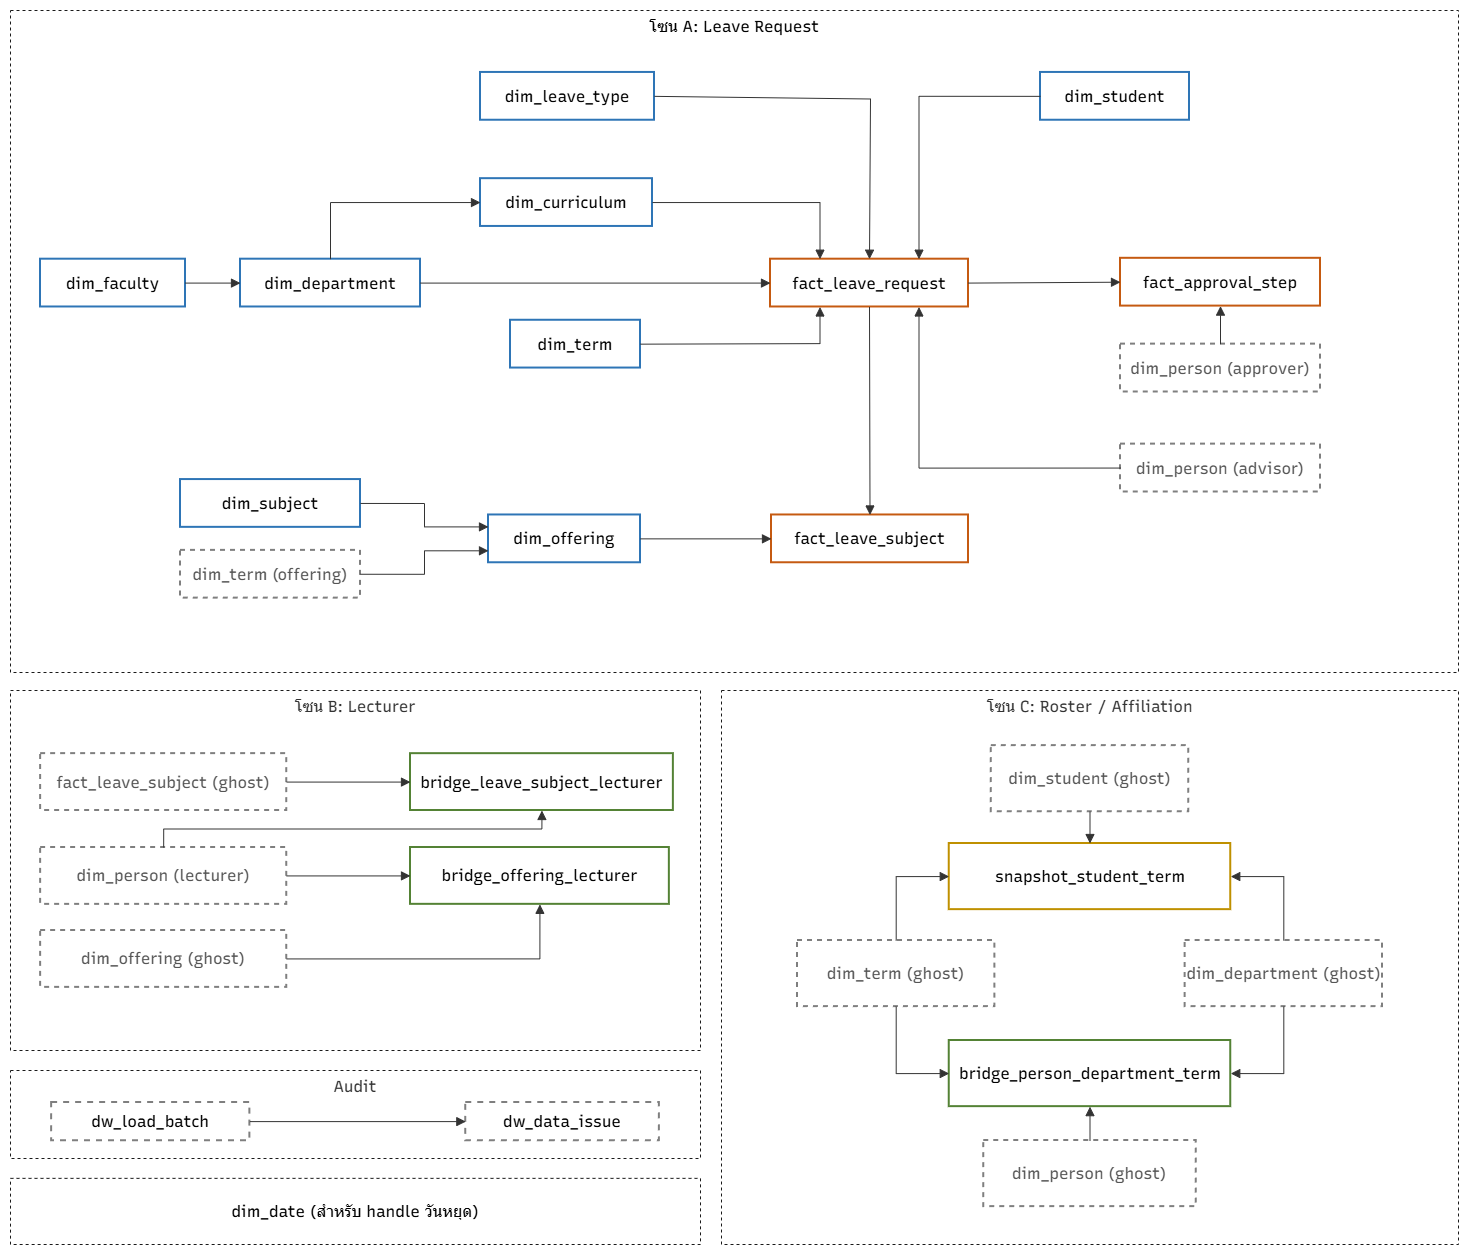
\includegraphics[width=\linewidth,height=0.68\textheight,keepaspectratio]{leave-schema/DW-OVERVIEW.png}
  \caption{ภาพรวมกลุ่มตารางคลังข้อมูลจากชุดภาพต้นฉบับ}
  \label{fig:warehouse-schema-overview}
\end{figure}
\clearpage
\begin{landscape}
  \subsection{ความสัมพันธ์ของข้อเท็จจริงและมิติ}
  คีย์ใบลาเชื่อมรายละเอียดรายวิชา ขณะที่คีย์นิสิต เทอม ประเภทลา และหน่วยงานใช้จัดกลุ่มข้อมูล ต้องรักษาระดับรายละเอียดของแต่ละตารางเมื่อรวมยอด
  \begin{figure}[H]
    \centering
    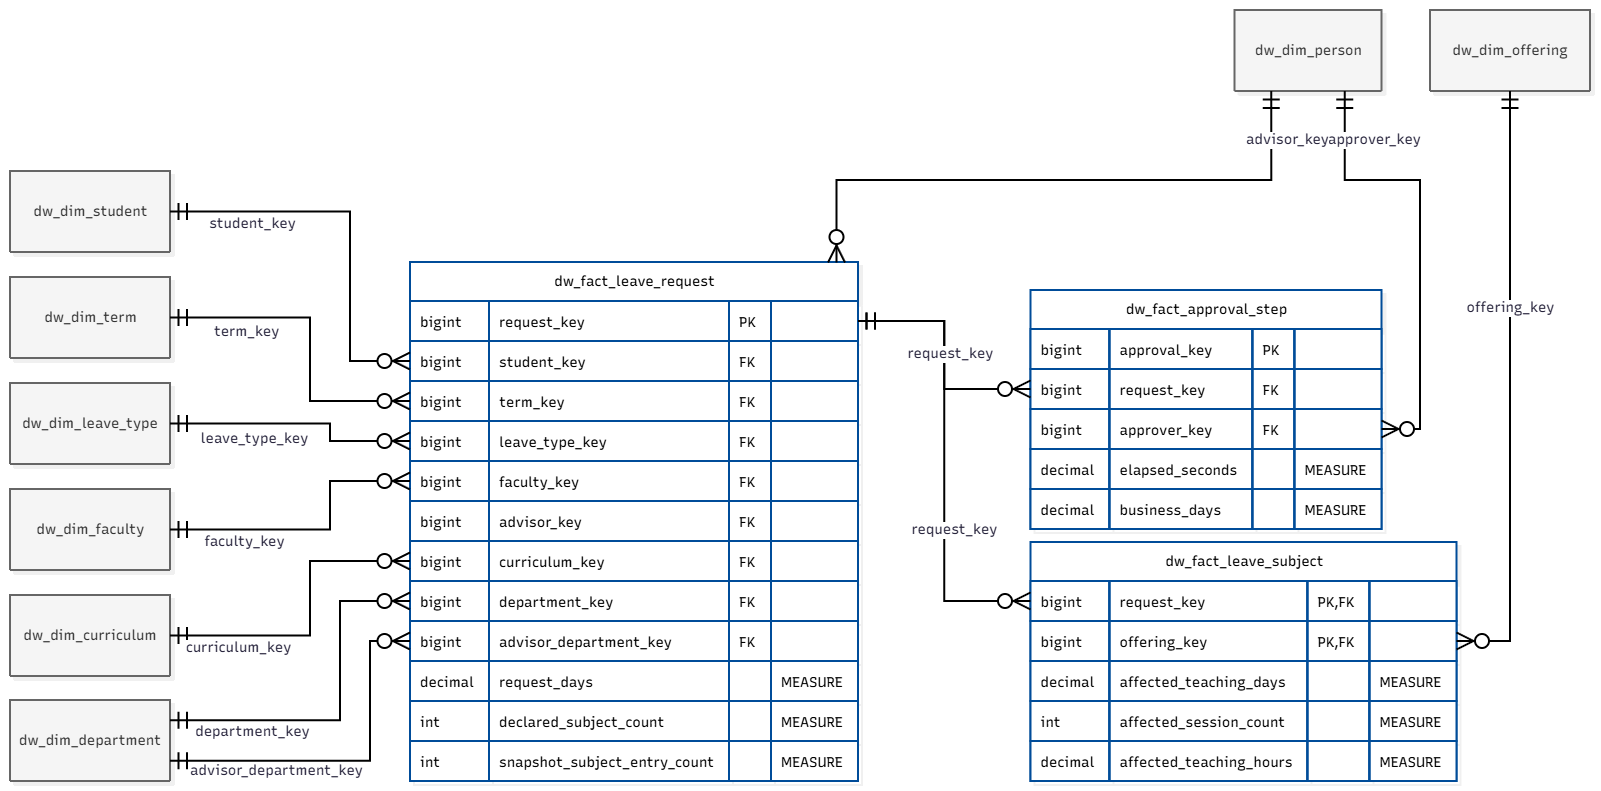
\includegraphics[width=\linewidth,height=0.74\textheight,keepaspectratio]{leave-schema/DW-ERD.png}
    \caption{ERD ของข้อเท็จจริงและมิติหลักในคลังข้อมูล}
  \end{figure}
\end{landscape}
\clearpage
\begin{landscape}
  \subsection{สคีมารุ่น 2 แบบเต็ม}
  ภาพแสดงชนิดคอลัมน์ คีย์หลัก และคีย์นอกของแบบจำลอง โดยแยกสีตามหน้าที่ของตาราง ใช้ประกอบคำอธิบาย fact ระดับใบลาและระดับใบลา--กลุ่มเรียนในบทที่ 3
  \begin{figure}[H]
    \centering
    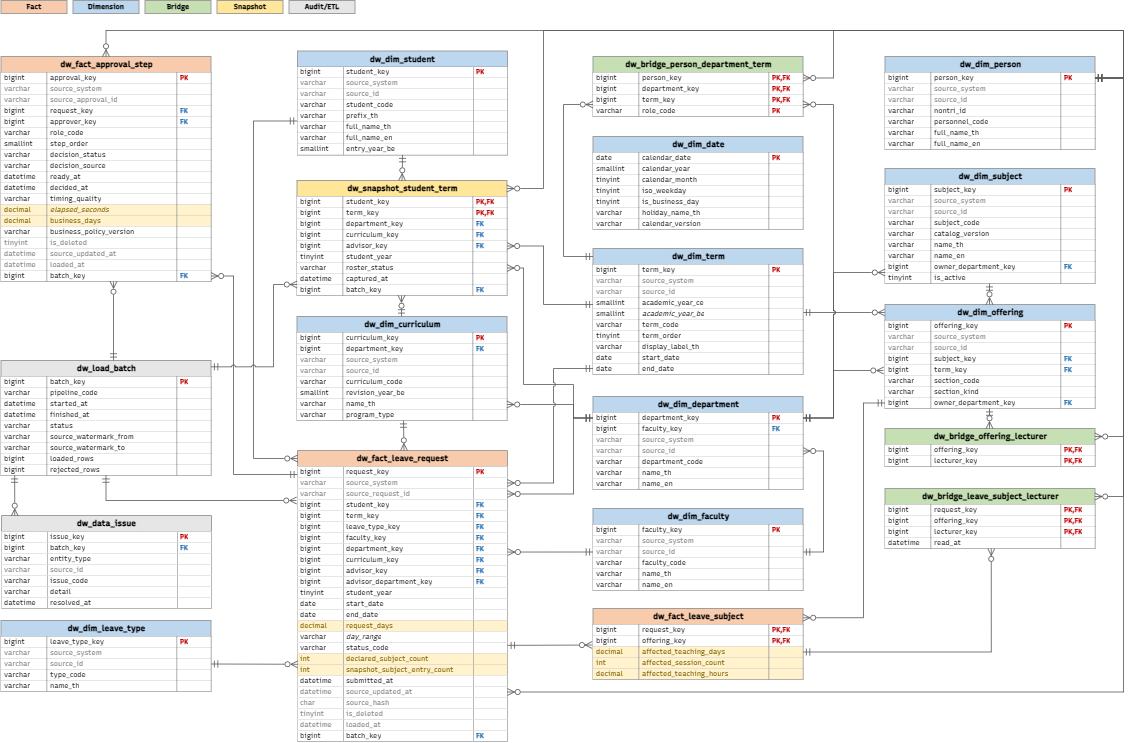
\includegraphics[width=\linewidth,height=0.74\textheight,keepaspectratio]{leave-schema/DW-FULL_VERSION_2.png}
    \caption{สคีมาคลังข้อมูลรุ่น 2: Fact, Dimension, Bridge, Snapshot และ Audit/ETL}
  \end{figure}
\end{landscape}
\clearpage
\begin{landscape}
  \subsection{คอลัมน์ควบคุมและตรวจสอบ ETL}
  รหัสระบบต้นทางและรหัสรายการช่วยระบุตัวตนข้อมูล ส่วน batch key เชื่อมข้อมูลกับรอบ ETL ตารางรอบนำเข้าและรายการปัญหาช่วยตรวจสอบการโหลดและติดตามคุณภาพข้อมูล
  \begin{figure}[H]
    \centering
    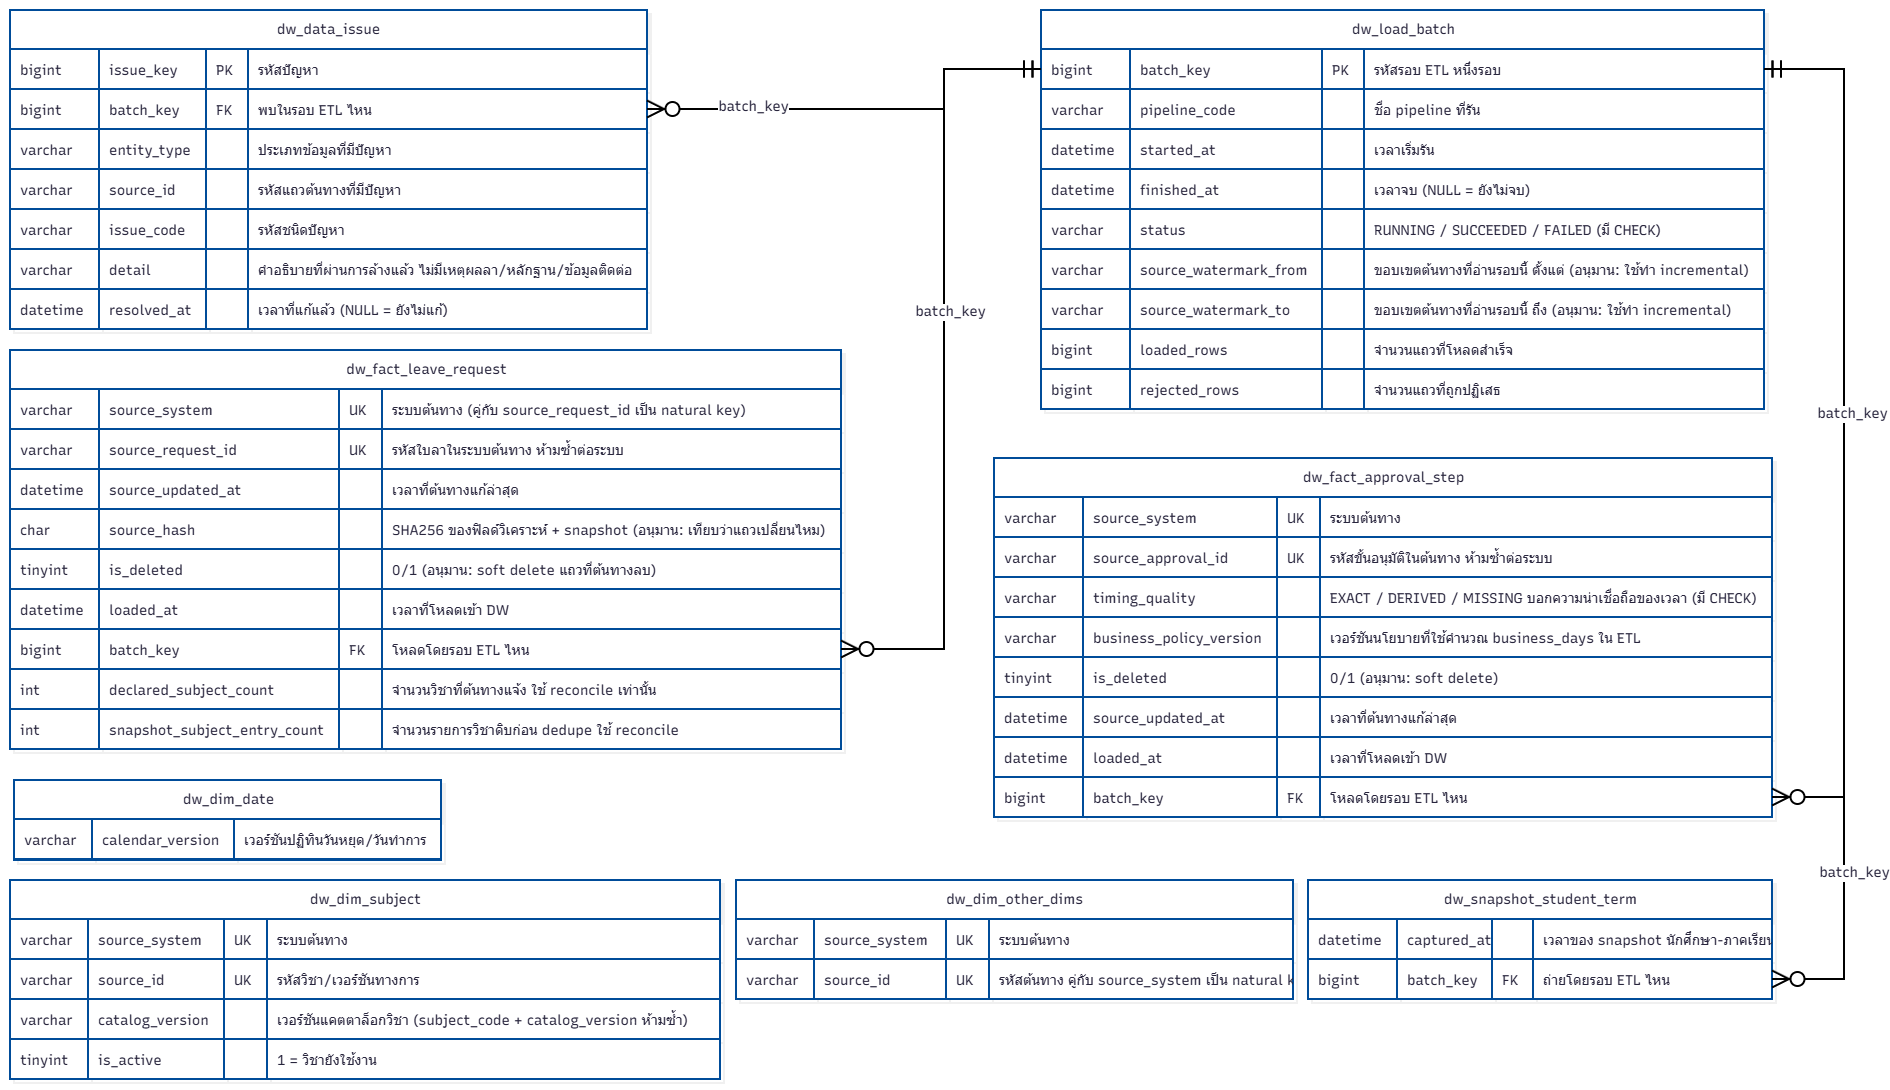
\includegraphics[width=\linewidth,height=0.74\textheight,keepaspectratio]{leave-schema/DW-CONTROL_COLUMNS.png}
    \caption{คอลัมน์อ้างอิงต้นทาง รอบนำเข้า และการตรวจสอบคุณภาพข้อมูล}
  \end{figure}
\end{landscape}
\clearpage

\end{document}
